\setlength{\footskip}{8mm}
\chapter{ Literature Review } \label{sec:literature}
This chapter describes the relevant literature for detecting road lanes and also the literature for the algorithms used in this thesis. 

\section{Road lane detection} 
\fullcite{McCall_videobased} provided an extensive survey of a number of
techniques for road lane detection as well as tracking. One of the observation 
made in this paper was that most of the techniques had a common flow; these 
were:
\begin{itemize}
\item Road Modeling - The parabolic or spline based road model is a good model 
for modeling both straight and curved lane marking. However one must take into 
account the environment that the system is to be used as well. For example on 
the highway it may be better to assume that the lane marking are straight and 
are parallel to simplify the problem. Figure \ref{fig:poor_edge_detection}(a) shows image with markings cause by tires while the lane marking on the right side in Figure \ref{fig:poor_edge_detection}(b) are not clearly visible and the two lanes differ in color. 
\item Road Marking Extraction - A lot of the papers in this survey used edge 
detection to extract the lane marking. Edge detection can work quite well but 
they fail when the roads other line markings or shadows. 
\begin{figure}
  \centering
  \begin{tabular}{c c}
    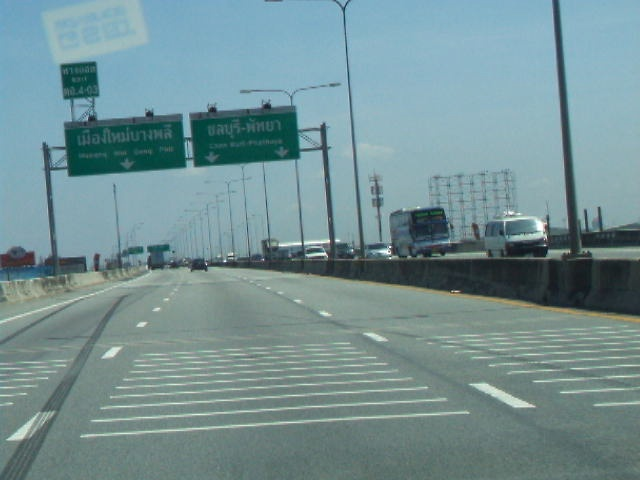
\includegraphics[width=60mm]{figures/edge1.jpg} &
    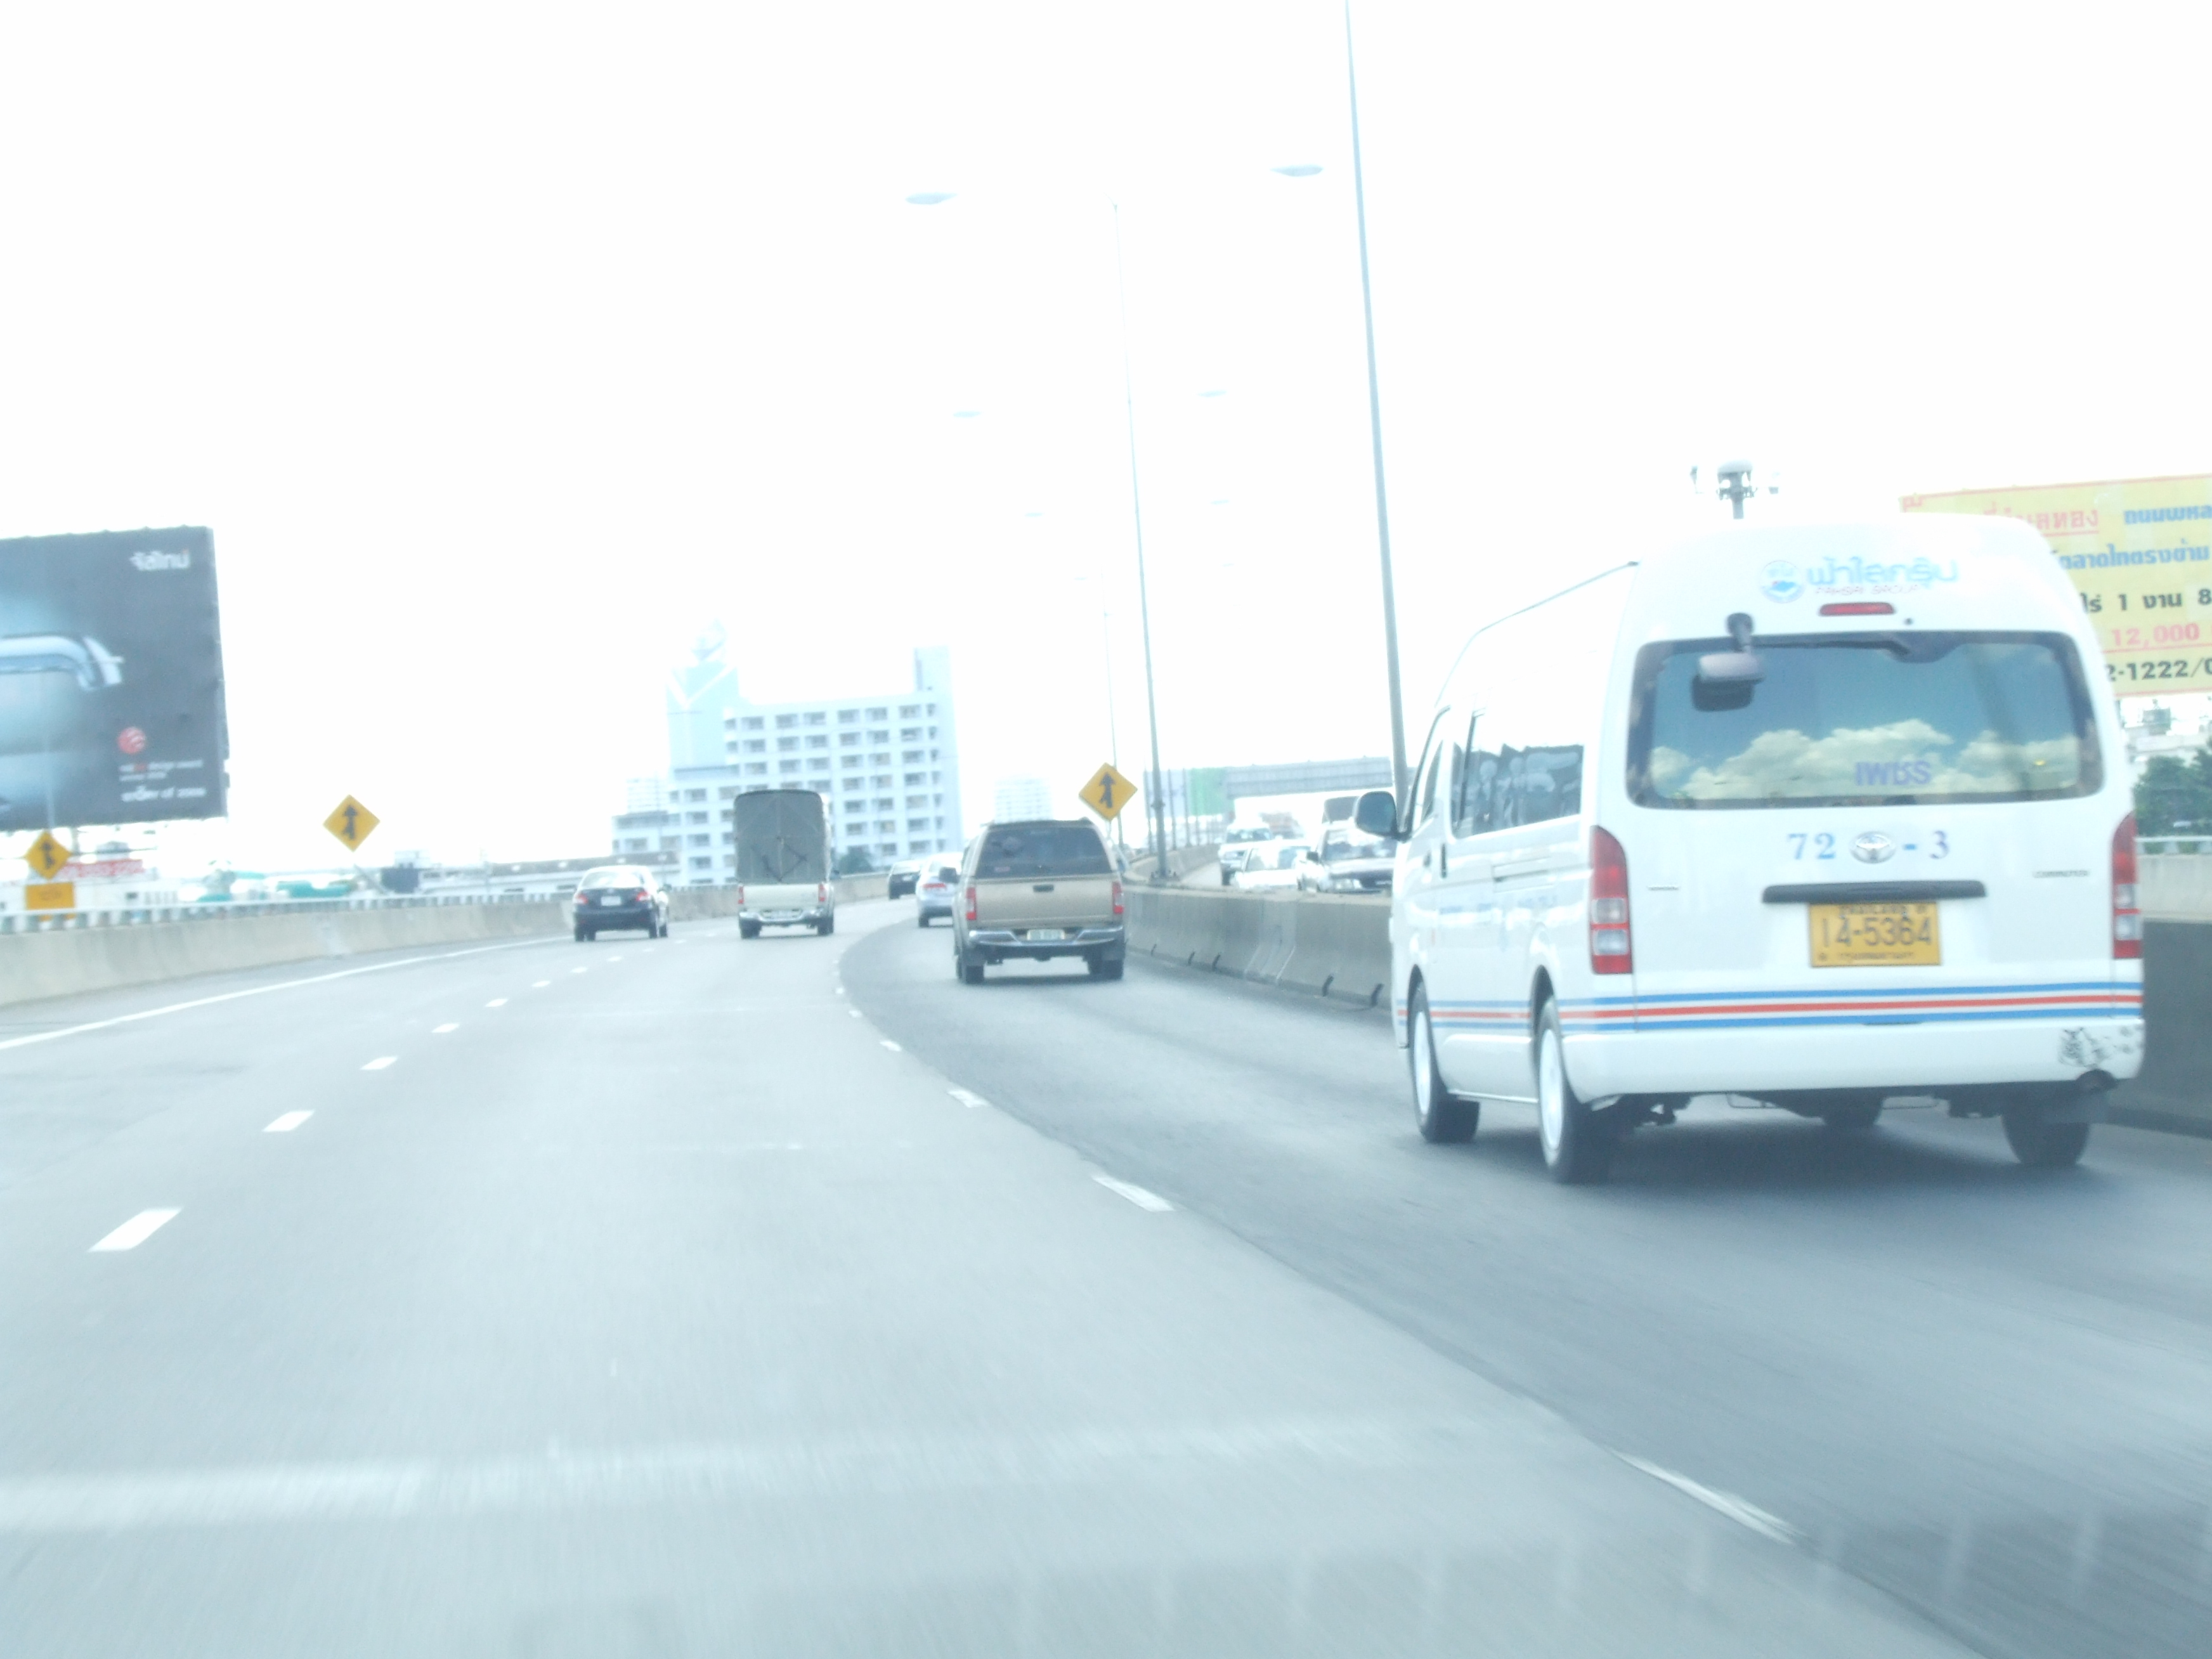
\includegraphics[width=60mm]{figures/edge2.jpg} \\
    (a) & (b) \\
  \end{tabular}
  \caption{Scenes where edge detection would perform poorly}
  \label{fig:poor_edge_detection}
\end{figure}
\item Post processing - Post processing is used to improve the estimated road 
lane marking that has been extracted. Hough transform was the commonly used 
technique.  
\item Vehicle Post processing and Tracking - Kalman filtering and particle 
filtering were the most common tracking techniques. Although not yet 
implemented. I plan to implement a Kalman filtering for tracking the road lanes. 
\end{itemize}


Another popular area in which road lane detection is used is autonomous vehicle. 
\fullcite{huang2008rss} proposed two algorithm for detecting road lanes which 
was used by the MIT team in the 2007 DARPA Urban Challenge. The first was baed 
on convolution of an image row with a matched filter while the second involved 
detection of symmetric contours which involved a lot of image processing. In 
this thesis I've implemented the first algorithm due to it's simplicity and low 
amount of computation.

In recent years there has been an interest to develop systems that are real time 
and can be implemented on embedded systems in which resources are limited. 
\fullcite{Hsiao20092089} developed a lane departure warning system using a 
combination of ARM based CPU and FPGA. The CPU was used for co-ordination of 
various image processing modules that was implemented on the FPGA. They were 
able to process 25 frames/s with each frame of size 256 $\times$ 256. The 
algorithm also performed reasonably well at night. The night time conditions was 
as good as the day time conditions. However they were able to detect only lane 
marking that was straight and therefore the decision of lane departure warning 
was based on lanes that were close to the car. \fullcite{Marzotto2010} also 
developed a lane departure warning system using an FPGA. Their system was more 
robust than \fullcite{Hsiao20092089} by using only an FPGA and processing up to 
30 frames/s each of size 752 $\times$ 480. The techniques used for detecting the 
road lanes were mostly common image processing techniques. Using a parabolic 
model similar to \fullcite{Kluge1994109} they were able to detect curved lane 
marking. 


Most of the road lanes detection only worked during the day time condition some 
worked at night as well but the system had to reconfigured. 
\fullcite{Wang2010113} proposed a system that would work at different lighting 
condition. The system used a fuzzy C-mean and fuzzy rule system to adjust the 
luminance which would adjust the threshold in the system and thereby allowing 
the system to produce the same result as the car is moving from day to dawn. 

On the industrial side, automobiles manufacturer such as Mercedes-Benz, Volvo
and Nissan claim to have built system for lane departure warning system. Some
of the recent cars produced by these manufactures also come with a lane
departure warning system pre-installed. For example the Mercdedes-Benz 
E-Class\fullcite{Mercedes} comes pre-installed with a system called "Lane 
Keeping Assist" which vibrates the steering wheel whenever the vehicle is about 
to leave the lane. At the time of this writing they have been no technical 
papers published by these manufactures describing their algorithm. However all 
these manufactures seems to be using a front-facing
camera to capture the roads view.


\section{RANSAC}
Random Sample Consensus or RANSAC\fullcite{RANSAC} is a technique is for 
estimating inliers from a set which contains both inliers and outliers. The 
following describes the generic algorithm for RANSAC.

Given a set $S$ than contains both inliers and outliers.
\begin{enumerate}
\item Randomly select a sample $s$ from $S$ so that the model can be
instantiated.
\item For every other data points in $S$ but not in $s$. If the point is within
the threshold $t$ then add the point the set of consensus set $S_{i}$. 
\item If $S_{i}$ is greater than some threshold $T$ then reestimate the model
with the points in $S_{i}$ and terminate else repeat step 1. 
\item Repeat steps 1 - 4 for $N$ trials the largest consensus set $S_{i}$ is
selected as the set with most inliers. 
\end{enumerate}

RANSAC has many application for example line fitting, circle fitting, ellipsoid 
fitting or any other mathematical model that needs to be estimated from a data 
set that contains outliers. For example if a road lane is modeled as a line 
RANSAC can be used to improve the estimate of the detected lane by removing the 
outliers. 

\section{Camera Calibration}
\label{sec:camera_calibration}
A image taken by the camera converts a 3D scene to a 2D image but often time we 
want to calculate the 3D point in the real world given a 2D point in the image. 
Using homogenous coordinates, the relationship between a 3D point in the real 
world $\vec{X} = [x\ \ y\ \ z\ \ 1]^T$ and a 2D point $\vec{x} = [x\ \ y\ \ 
1]^T$ on the image plane can be expressed as: 
\begin{equation}
  \label{eq:camera_equation}
  \vec{x} \sim \vec{P}\vec{X}
\end{equation} 
where $\mat{P}$ is a $3 \times 4$ homogenous camera matrix that consists of the 
intrinsic and extrinsic parameters which can be expressed as: 
\begin{equation}\vec{P} = \mat{K}[\mat{R}\mid\vec{t}]\end{equation} \label{eq:camera_equation_2}
where $\mat{K}$ is the camera calibration matrix consisting of the intrinsic 
parameters
$$\mat{K} = \begin{bmatrix}f&s&p_{x}\\&f&p_{y}\\&&1\end{bmatrix}$$
while $\mat{R}$ is a $3 \times 3$ rotational matrix and $\vec{t}$ is the 
translation vector from the world to the camera coordinate system. 
